% Drawing 33/09-7 -- folder 33, batch 09, archive page 179 (PDF page 180).
% Transcription: sous trois des termes de la seconde ligne, des flèches verticales vers $A$ ; sous la première, l'annotation « dualité parfaite triviale (via \uncertain{pureté} …) » ; sous les deux autres, réunies par des arcs, « dualité parfaite ?? ».
% Kind: vertical arrows under terms of an exact sequence, with annotations. Method 2 (schematic redraw from the facsimile). Status: ok.
% Notes: Under three terms of the second line (written above; the line is text and not redrawn): two arrows down to A, and under the third a plain vertical stroke down to A (no arrowhead on the page). Left of the first A, a bracket; under it, on four lines, "dualité parfaite triviale (via pureté ...)". The second and third columns are joined by two arcs that come down together towards "dualité parfaite ??" (no arrowheads on the page; the earlier redraw gave them heads). Annotations placed as written. Redrawn 2026-11-09 (issue 128): to check again.
% Coordinates: 1 unit = 1 mm = 1/100 of the crop width (bbox in page fractions: [0.05, 0.12, 0.75, 0.37]).
% Redrawn by Claude (claude-opus-5-5), issue #73, 2026-11-09; not checked by a human; not compiled (no TeX in the session).
% Rights: reproduces part of the work -- behind RENDER_TRANSCRIPTS, never published by itself.
\documentclass[tikz,border=3pt]{standalone}
\usepackage{amsmath,amssymb}
\usetikzlibrary{patterns,arrows.meta}
\tikzset{pencil/.style={black!45}, struck/.style={black!35}, mark/.style={circle,draw,inner sep=1.3pt}, pt/.style={circle,fill,inner sep=0.9pt}, opt/.style={circle,draw,fill=white,inner sep=1.1pt}}
\begin{document}
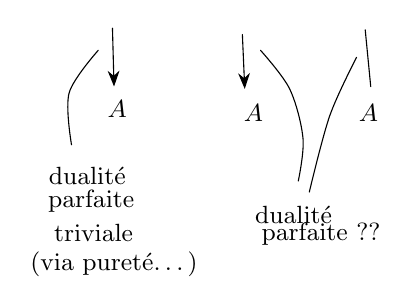
\begin{tikzpicture}[x=1mm,y=1mm,line cap=round,line join=round,font=\scriptsize]
\draw[-{Stealth[length=2mm]}] (54.1,-16.9) -- (54.3,-24.3);
\draw[-{Stealth[length=2mm]}] (70.6,-17.7) -- (70.9,-24.6);
\draw (86.2,-17.1) -- (86.9,-24.3);
\node[inner sep=1pt] at (54.7,-27.1) {\small $A$};
\node[inner sep=1pt] at (72,-27.7) {\small $A$};
\node[inner sep=1pt] at (86.6,-27.7) {\small $A$};
\draw plot[smooth, tension=0.55] coordinates {(52.3,-19.7) (48.6,-25.1) (48.9,-31.7)};
\draw plot[smooth, tension=0.55] coordinates {(72.9,-19.7) (76.6,-24.6) (78.3,-30.9) (77.7,-36.3)};
\draw plot[smooth, tension=0.55] coordinates {(85.1,-20.6) (81.7,-28) (79.1,-37.7)};
\node[inner sep=1pt] at (50.9,-35.7) {\small dualité};
\node[inner sep=1pt] at (51.4,-38.9) {\small parfaite};
\node[inner sep=1pt] at (51.7,-42.9) {\small triviale};
\node[inner sep=1pt] at (54.3,-46.9) {\small (via pureté\dots)};
\node[inner sep=1pt] at (77.1,-40.6) {\small dualité};
\node[inner sep=1pt] at (80.6,-43.1) {\small parfaite ??};
\end{tikzpicture}
\end{document}
